% -*- latex -*-

%%%%%%%%%%%%%%%%%%%%%%%%%%%%%%%%%%%%%%%%%%%%%%%%%%%%%%%%%%%%%%%%%%%%%%%%%%%%%
% This beginning part of the preamble is psecific to the IEEEtran document
% class.

\documentclass[conference]{IEEEtran}

%% \author{
%%   \IEEEauthorblockN{Kenneth~Moreland}
%%   \IEEEauthorblockA{Sandia National Laboratories\\
%%     Albuquerque, NM 87185-1326\\
%%     Email: kmorel@sandia.gov}
%%   \and
%%   \IEEEauthorblockN{Others}
%%   \IEEEauthorblockA{Cool Group\\
%%     Somewhere, WQ 12341\\
%%     Email: person@myspace.com}
%% }

\author{
  \IEEEauthorblockN{
    Kenneth~Moreland\IEEEauthorrefmark{1}
  }
  \IEEEauthorblockA{
    \IEEEauthorrefmark{1}Sandia National Laboratories,
    Albuquerque, NM 87185-1326}
}

% for over three affiliations, or if they all won't fit within the width
% of the page, use this alternative format:
%
%\author{\IEEEauthorblockN{Michael Shell\IEEEauthorrefmark{1},
%Homer Simpson\IEEEauthorrefmark{2},
%James Kirk\IEEEauthorrefmark{3},
%Montgomery Scott\IEEEauthorrefmark{3} and
%Eldon Tyrell\IEEEauthorrefmark{4}}
%\IEEEauthorblockA{\IEEEauthorrefmark{1}School of Electrical and Computer Engineering\\
%Georgia Institute of Technology,
%Atlanta, Georgia 30332--0250\\ Email: see http://www.michaelshell.org/contact.html}
%\IEEEauthorblockA{\IEEEauthorrefmark{2}Twentieth Century Fox, Springfield, USA\\
%Email: homer@thesimpsons.com}
%\IEEEauthorblockA{\IEEEauthorrefmark{3}Starfleet Academy, San Francisco, California 96678-2391\\
%Telephone: (800) 555--1212, Fax: (888) 555--1212}
%\IEEEauthorblockA{\IEEEauthorrefmark{4}Tyrell Inc., 123 Replicant Street, Los Angeles, California 90210--4321}}

% End of IEEEtran-specific portion of the preamble.
%%%%%%%%%%%%%%%%%%%%%%%%%%%%%%%%%%%%%%%%%%%%%%%%%%%%%%%%%%%%%%%%%%%%%%%%%%%%%


\usepackage{amsfonts}
\usepackage{amssymb}
\usepackage{amsmath}
\usepackage{booktabs}
\usepackage{graphicx}
\usepackage{varioref}
\usepackage{fancyvrb}
\usepackage{ifthen}
\usepackage{cite}
\usepackage{subfig}
\usepackage{xspace}
\usepackage[pdfborder={0 0 0}]{hyperref}
\usepackage{verbatim}

\usepackage{color}
\definecolor{yellow}{rgb}{1,1,0}
\definecolor{black}{rgb}{0,0,0}
\definecolor{ltcyan}{rgb}{.75,1,1}
\definecolor{red}{rgb}{1,0,0}
\definecolor{gray}{rgb}{.6,.6,.6}
\definecolor{darkred}{rgb}{0.5,0,0}
\definecolor{darkgreen}{rgb}{0,0.5,0}

\definecolor{goodcolor}{rgb}{0.1,0.1,0.8}
\definecolor{badcolor}{rgb}{0.86,0.08,0.24}

% Cite commands I use to abstract away the different ways to reference an
% entry in the bibliography (superscripts, numbers, dates, or author
% abbreviations).  \scite is a short cite that is used immediately after
% when the authors are mentioned.  \lcite is a full citation that is used
% anywhere.  Both should be used right next to the text being cited without
% any spacing.
\newcommand*{\lcite}[1]{~\cite{#1}}
\newcommand*{\scite}[1]{~\cite{#1}}

\newcommand{\etal}{et al.}

\newcommand{\insitu}{{\it in situ}\xspace}
\newcommand{\intransit}{{\it in transit}\xspace}

\newcommand*{\keyterm}[1]{\emph{#1}}

\newcommand{\fix}[1]{{\color{red}\textsc{[#1]}}}

% Avoid putting figures on their own page.
\renewcommand{\textfraction}{0.05}
\renewcommand{\topfraction}{0.95}
\renewcommand{\bottomfraction}{0.95}

% Make sure this is big enough so that only big figures end up on their own
% page but small enough so that if a figure does have to be on its own
% page, it won't push everything to the bottom because it's not big enough
% to have its own page.
\renewcommand{\floatpagefraction}{.75}

\title{Oh, \$\#*@! Exascale! The Effect of Emerging Architectures on
  Scientific Discovery}

% I hacked up IEEEtran.cls to support a teaser for conference papers.
\newcommand{\teaser}{
  \centering
  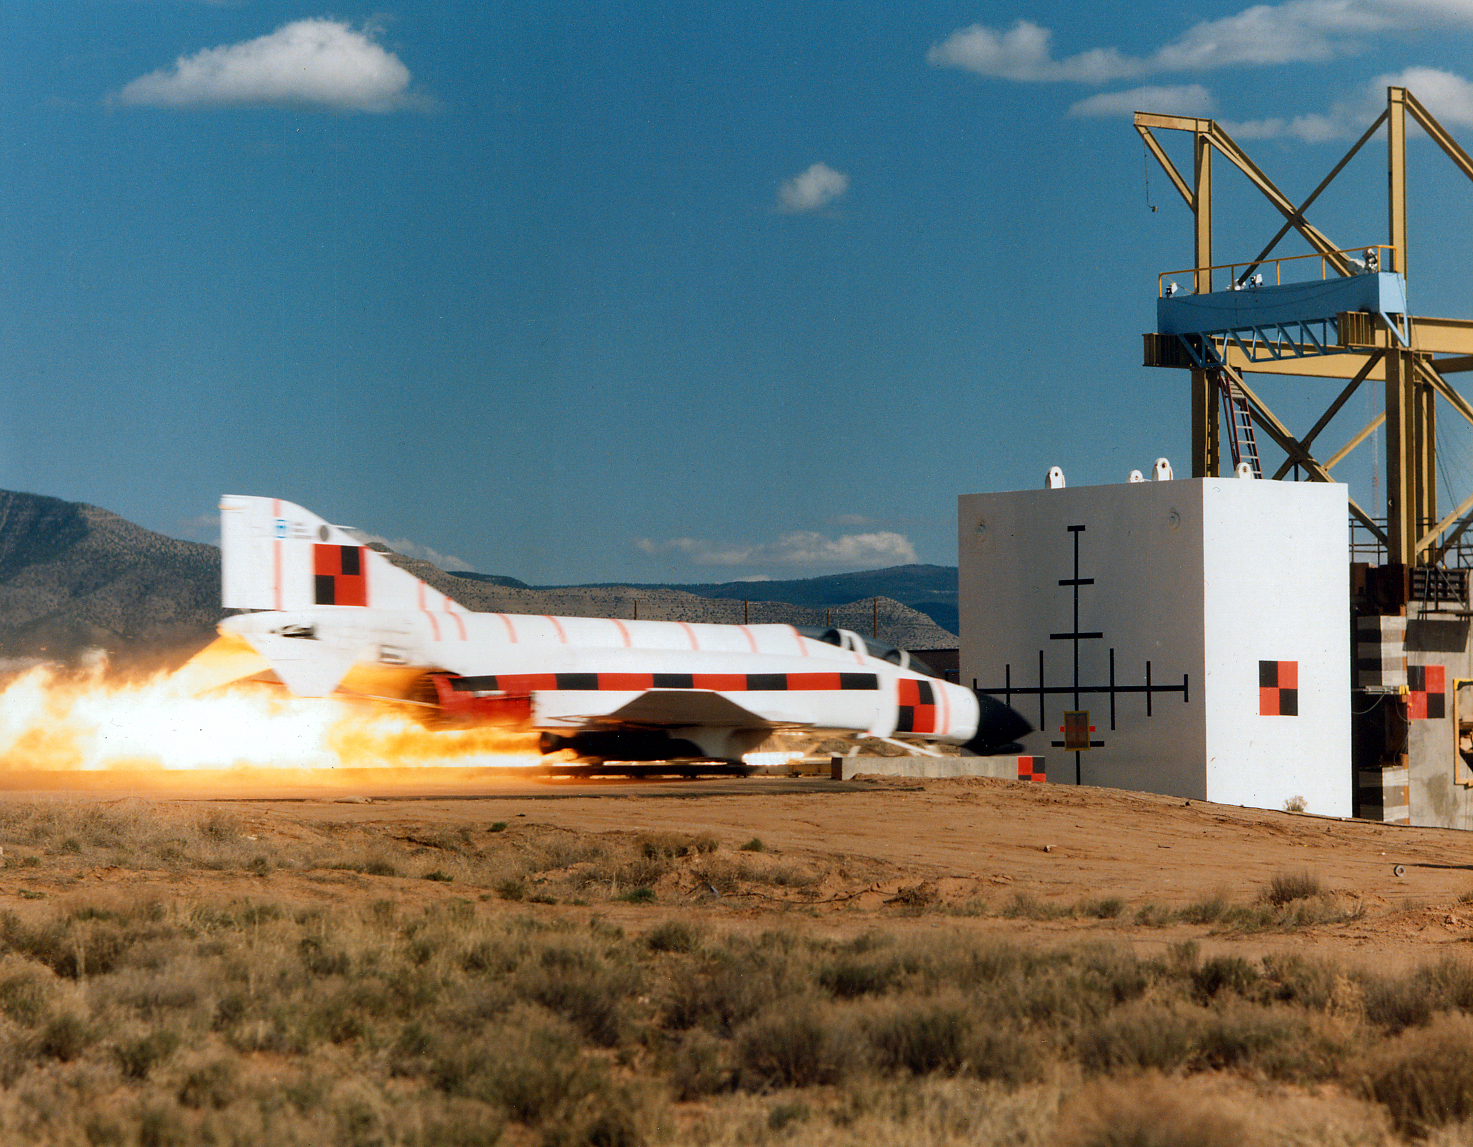
\includegraphics[height=1.8125in]{images/Rocket1}
  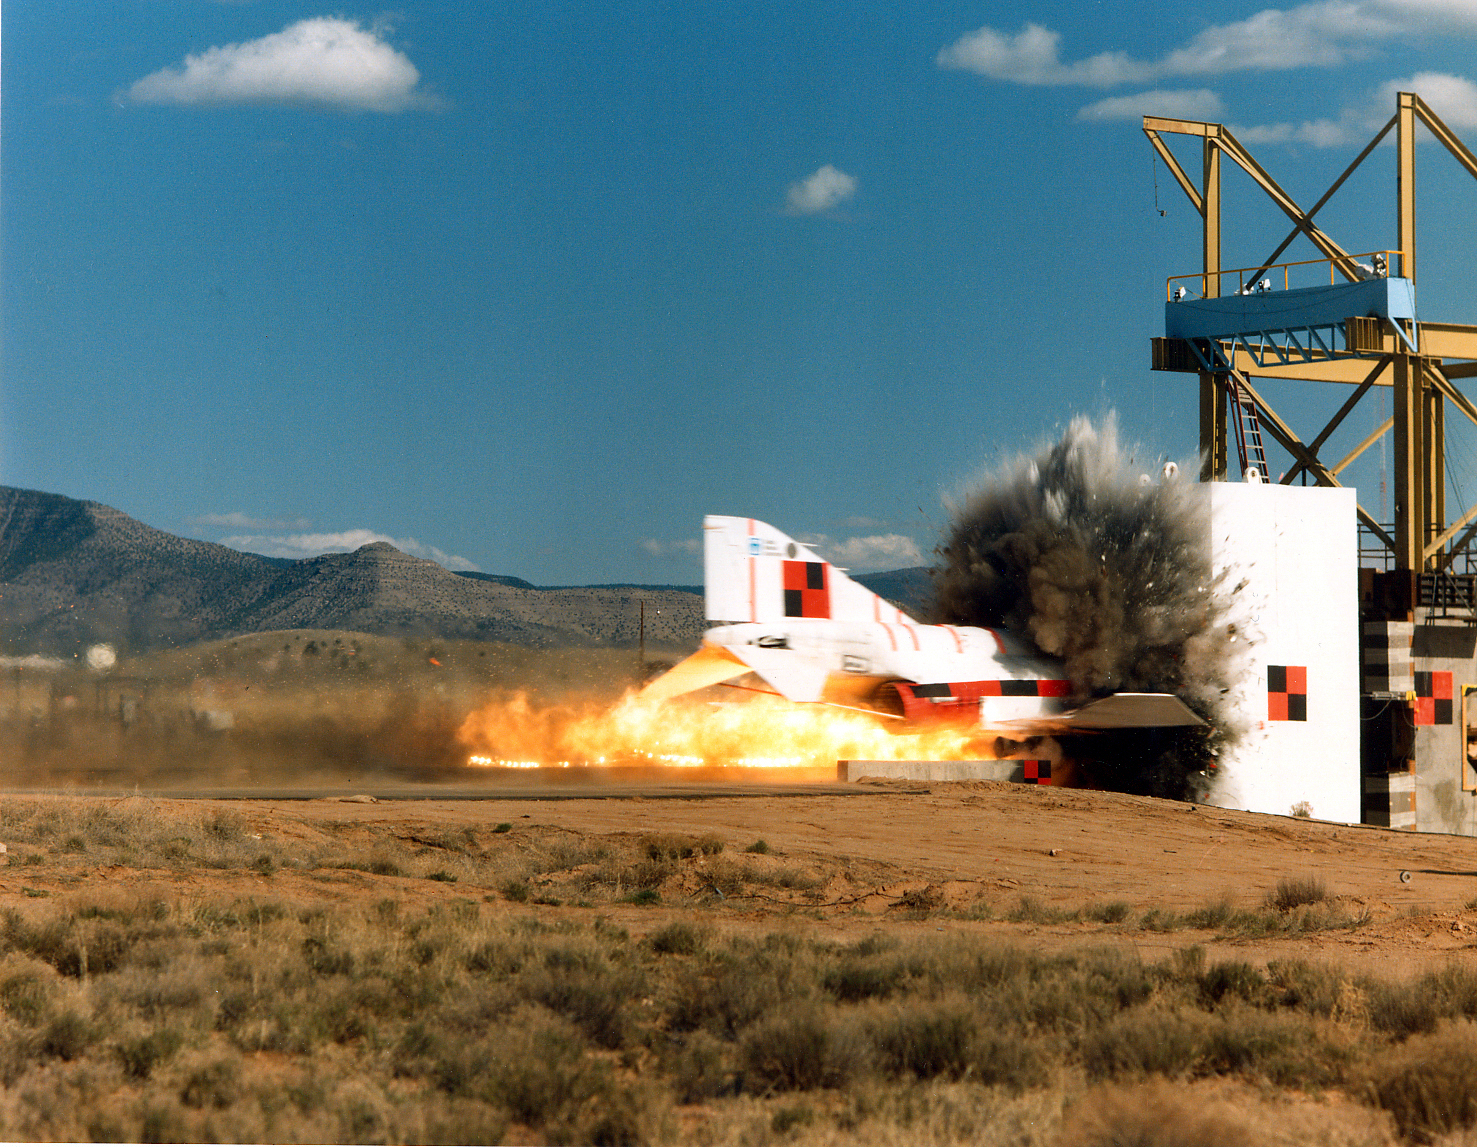
\includegraphics[height=1.8125in]{images/Rocket2}
  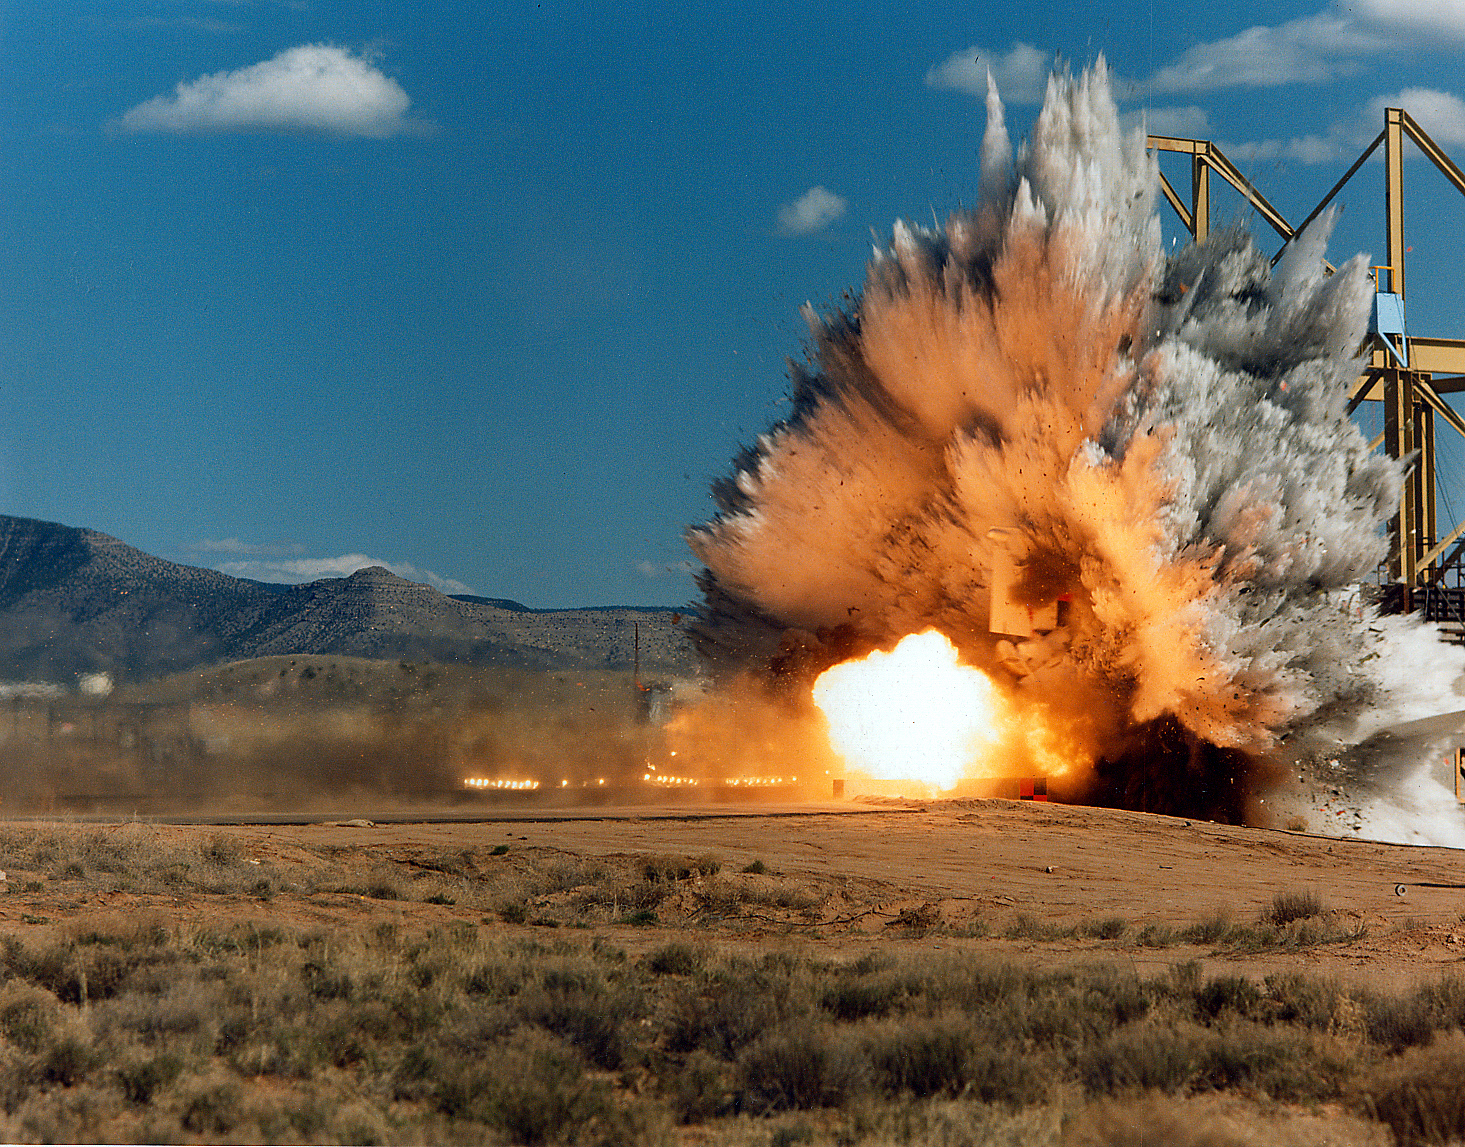
\includegraphics[height=1.8125in]{images/Rocket3}
  \caption{This 1988 rocket-sled test has nothing to do with exascale
    computing per se, but it makes for an effective metaphor for the
    ``brick wall'' we anticipate our high-performance computing code to
    collide with.}
  \label{fig:teaser}
}

\begin{document}

\sloppy

\maketitle

\begin{abstract}
The predictions for exascale computing are dire.  Although we have
benefited from a consistent supercomputer architecture design, even across
manufacturers, for well over a decade, recent trends indicate that future
high-performance computers will have different hardware structure and
programming models to which software must adapt.  This paper provides an
informal discussion on the ways in which changes in high-performance
computing architecture will profoundly affect the scalability of our
current generation of scientific visualization and analysis codes and how
we must adapt our applications, workflows, and attitudes to continue our
success at exascale computing.
\end{abstract}

\section{Introduction}
\label{sec:Introduction}

\noindent
Thanks to recent advances in parallel visualization algorithms and
frameworks, we currently benefit from production large-scale
scientific-visualization applications such as ParaView\lcite{ParaView} and
VisIt\lcite{VisIt}, which are shown to be very scalable up to our current
generation of petascale computers\lcite{Childs2010}.  Although the
development of these tools comes from the successful scaling of techniques
originally pioneered over ten years ago\lcite{Ahrens2000,Wylie2001}, recent
trends indicate that future high-performance computers will have different
hardware structure and programming models to which software must adapt.

These grave predictions come from multiple
workshops\lcite{ExascaleArchitecturesReport,ExascaleRoadMap,DARPAExascaleStudy}
where experts convened to discuss the roadmap to building exascale
computers (that is, computers capable of performing $10^{18}$ floating
point operations per second).  Table~\ref{table:PetascaleVsExascale} gives
a summary comparison between an existing petaFLOP computer and the expected
system performance of a future computer capable of an exaFLOP.  Note that
there is uncertainty in what type of computer architecture will be used to
achieve an exaFLOP (and it is possible different architectures may be used
in different instances).  To compensate for this uncertainty, experts use
the term design ``swim lanes'' that capture these different approaches.
Two likely swim lanes are captured in
Table~\ref{table:PetascaleVsExascale}.

If all the components of supercomputers were to be scaled uniformly, then
the ``Factor Change'' column in Table~\ref{table:PetascaleVsExascale} would
have uniform values.  However, the factor of change varies wildly from very
small changes to five orders of magnitude.  The main cause for most of this
variability comes from compromises made to achieve the desired system peak
(the first column of Table~\ref{table:PetascaleVsExascale}) with the
constraints of a limited power budget (the second column of
Table~\ref{table:PetascaleVsExascale}).  DOE has established a power budget
for the exascale machine at 20~MW\lcite{ExascaleArchitecturesReport}.  The
reason for this budget is very pragmatic.  The operating cost of a
supercomputer is roughly \$1 million per megawatt per year.  As such, DOE
determines that it cannot afford more than \$20 million per year to operate
a single supercomputer.  Thus, the challenge of exascale computing is
getting about three orders of magnitude improvement in computation rate
using not much more power than we do today.

\begin{table*}[htdp]
  \centering
  \caption{Comparison of a petascale supercomputer to an expected exascale
    supercomputer\lcite{ScientificDiscoveryExascale2011}.}
  \label{table:PetascaleVsExascale}
  \begin{tabular}{@{}lcccc@{}}
    \toprule
    & & \multicolumn{2}{c}{Exascale (Prediction)} & \\
    System Parameter & Petascale & Swim Lane 1 & Swim Lane 2 & Factor Change \\
    \midrule
    System Peak & 2 Pf/s & \multicolumn{2}{c}{1 Ef/s} & 500 \\
    Power & 6 MW & \multicolumn{2}{c}{$\le$20 MW} & 3\\
    System Memory & 0.3 PB & \multicolumn{2}{c}{32--64 PB} & 100--200 \\ % San Diego report says 50PB
    Total Concurrency & 225K & 1B$\times$10 & 1B$\times$100 & 40,000--400,000 \\
    Node Performance & 125 GF & 1 TF & 10 TF & 8--80\\
    %Node Memory BW & 25 GB/s & 400 GB/s & 4 TB/s & 16 \\
    Node Core Count & 12 & 1,000 & 10,000 & 83--830 \\
    Network BW & 1.5 GB/s & 100 GB/s & 1000 GB/s & 66--660 \\
    System Size (nodes) & 18700 & 1,000,000 & 100,000 & 50--500 \\
    I/O Capacity & 15 PB & \multicolumn{2}{c}{300--1000 PB} & 20--67\\
    I/O BW & 0.2 TB/s & \multicolumn{2}{c}{20--60 TB/s} & 10--30 \\
    \bottomrule
  \end{tabular}
\end{table*}

Using the predictions in Table~\ref{table:PetascaleVsExascale}, this paper
provides an overview of the changes required to our scalable code and how
we use our applications.  In particular, we will note the contrast between
the factor change of related system parameters and discuss the
implications.  This paper provides an informal discussion of these issues.
For a more formal discussion, consult the report from the DOE ASCR 2011
Workshop on Exascale Data Management, Analysis, and
Visualization\lcite{ScientificDiscoveryExascale2011}.

\section{Concurrency}
\label{sec:Concurrency}

\noindent
Let us first compare the amount of memory expected on our exascale machine
with the amount of concurrency programs will have to exhibit at scale.  The
system memory of the machine will grow by a factor of about a hundred,
which is an order of magnitude lower than than the growth of the
computational power.

The reason for this low growth of memory is that memory tends to be power
hungry.  Thus, we simply cannot afford to grow the amount of memory in the
system at a rate equal to the computation.  Furthermore, additional memory
does not directly contribute to the computational rate of the system.  Of
course, by that logic we could create an even cheaper exascale machine by
not adding or perhaps even removing some system memory.  However, doing so
would render the machine useless, and neither DOE nor any other
organization is willing to spend millions of dollars on a useless machine.
So, the amount of memory to be added to an exascale machine is an
engineering decision to maximize the utility of the system while keeping
everything in budget.

In contrast, the total concurrency required by the system will grow by up
to five orders of magnitude.  The reason for this staggering increase in
concurrency is twofold.  First, although Moore's law still holds for the
scaling of the number of transistors (so far), this scaling is no longer
contributing to the faster operation of processing
cores\lcite{ExascaleRoadMap}.  Instead, increased computing power is
achieved by adding more cores to a processor.  Given this fixed calculation
rate per core, we can predict that we will need roughly a billion cores to
sustain a rate of $10^{18}$ floating point operations per second.

Of course, the change in Moore's law only accounts for an increase of three
orders of magnitude.  The second factor that is increasing total
concurrency is the interface between the processor and the memory holding
the data it operates on.  Because the latency to off-chip memory is not
expected to improve substantially, practical applications will likely have
to run 10 to 100 threads per core (depending on the type of processor) to
hide this latency by swapping threads during memory
fetches\lcite{ExascaleArchitecturesReport}.  Consequently, a program could
require up to \emph{100 billion concurrent threads} to maintain an
exaFLOP.

\subsection{Scalability of Current Applications}

\noindent
This combination of low memory growth and high concurrency growth
represents serious scaling issues for our parallel high-performance
computation code.  Our current production scientific-visualization
applications use a distributed memory model with a message passing
interface, embodied in the use of MPI\lcite{MPI}, to implement concurrent
processing and communication.  Although this simple but effective model has
served well to the petascale era of supercomputing, it fails to capture
important emerging features in high-performance computing, and it is thus
doomed to break down unless major restructuring efforts are enacted.

To understand why our parallel production applications will fail to scale,
let us consider a simple and artificial but realistic and representative
example of performing scientific visualization on a regular grid of cells.
For a capability run on the petascale machine represented in
Table~\ref{table:PetascaleVsExascale} we could expect a grid of 1 trillion
cells\lcite{Childs2010}.  On the exascale machine, having about 100 times
more memory, we could expect a grid of 100 trillion cells.

Our current production scientific-visualization applications use MPI to
represent all concurrency, and MPI uses operating system processes to
represent concurrent execution.  Thus, to run on the entirety of a
petascale machine, an application would need about 200 thousand processes
whereas an exascale machine could require up to 100 billion processes.  One
problem with an operating system process is that it is a heavy weight
object.  Associated with each one is an entire program state including a
copy of the machine instructions to be executed.  A library of
general-purpose scientific visualization algorithms could be expected to
run at least 20~MB, and these 20~MB would have to be replicated on each
process.  Replicating this data 200 thousand times on the petascale machine
yields 4~TB, which is reasonable at less than 2\% of the overall memory
in the system.  However, replicating this data 100 billion times on the
exascale machine yields 2~EB, well over the amount of memory available on
the entire machine (and, incidentally, all of its storage).  Thus, we cannot
even start our application on the exascale machine, and that is before we
even load any data.

But let us say we get around that problem, which is an active area of
research\lcite{Balaji2011}.  Another problem that we run into is the
breakdown of Gustafson's law.  Scientific visualization code, as well as
most modern high-performance parallel code, gets around the limits of
parallel efficiency proposed by Amdahl\lcite{Amdahl1967} by scaling up the
problem size along with the concurrency\lcite{Gustafson1988}.  By
considering a scaled speedup, we can allow the problem size to be an
increasing function of the number of processes\lcite{Quinn2004}.  However,
limiting the growth of memory limits the scale to which we can grow
problems.

Back to our example, assuming that our visualization algorithm uses data
parallelism, which most modern visualization algorithms
do\lcite{Moreland2012:TVCG}, our 1 trillion cell petascale problem will be
broken into partitions of 5 million cells for each thread.  Experience
shows 5 million cells per thread to be an efficient amount to drive a
visualization pipeline thread\lcite{ParaViewTutorial}.  In contrast, the
equivalent exascale mesh of 100 trillion cells would be divided into
partitions of 1000 cells, a ridiculously small and inefficient amount to
overcome the overhead of a parallel program.

But even ignoring this problem, others abound.  Consider the issue of
adding ghost cells (or sometimes called halo cells) to our partitions.
Ghost cells are critical to the operation of our current parallel
scientific visualization algorithms; they limit the communication required
in the algorithms to make the parallel overhead manageable.  Assuming our
petascale problem is broken into 5 million cell partitions that are roughly
$171^3$ blocks, each block would require $6 \times 171^2$ or about 175
thousand ghost cells.  All total, this is 35 billion ghost cells, which
amounts to about 3.5\% of the original data size.  In contrast, our
exascale mesh would be broken into 1000 cell partitions of $10^3$ blocks,
and each block would require $6 \times 10^2 = 600$ ghost cells.  All total,
this is 60 trillion ghost cells, which amounts to about 60\% of the
original data size.  Growing the memory overhead by 60\% is simply not
feasible in most serious applications.

\subsection{Exascale Programming Challenges}

\noindent
These problems and many others plague our efforts to achieve scientific
discovery at exascale.  Simply put, at some point our current approach of
domain decomposition fails.  Eventually we require too many ghost cells,
too much communication, or simply have too fine of partitions to be
efficient.  What this means is that a significant portion of our code needs
to be redesigned and reimplemented.

In addition to revisiting and reengineering our scientific visualization
code, we must also cope with new, emerging, and conflicting architectures
and programming models.  The most blatant challenge is the proliferation of
compiler and libraries used to program these new multithreaded processors.
Currently popular technologies include OpenMP, CUDA, OpenCL, Intel
Threading Building Blocks, and OpenACC with many others also proposed and
available.  None of these solutions is universally available for all
hardware and all development environments, nor are any likely to become a
universal solution.  Thus, if a developer wants broad access to his or her
application, the code must be ported across significantly different
programming environments.

Furthermore, different hardware environments have their own idiosyncrasies
that must be taken into account above any basic compiler porting issues.
For example, a typical multicore CPU processor has a cache structure
optimized to provide independent memory access to each core.  This means
that memory must be divided along cache lines among cores to prevent
inefficiencies associated with issues such as false sharing\lcite{TBB}.  In
contrast, a GPU accelerator typically has cores grouped together in blocks
in which threads group memory fetches and share cache\lcite{Sanders2011}.
This differing organization of threads requires equally different
organization of scheduling and memory access within a program.

Eventually, scientific-visualization code must be reengineered using to use
an efficient shared-memory execution model (or more specifically, allow a
hybrid shared-distributed execution\lcite{Li2008}).  Although we have been
successful at implementing efficient, scalable distributed-memory
algorithms, writing algorithms in this threaded shared-memory environment
poses many challenges.  It is a common misconception that threaded
shared-memory programming is easier because it does not require the data
partitioning and message passing typically required for distributed-memory
programming.  This, however, is untrue because although distributed-memory
programming has a larger up-front cost of determining memory management and
communication, this design process inherently leads us to efficiently
structured code.  Proper partitioning is as important in shared memory as
in distributed memory, but threaded programming generally does not provide
the programmatic constraints to simplify and control the partitioning.
Furthermore, distributed memory models' isolation of memory spaces helps
prevent read-write collisions and deadlocks whereas any errant memory
access anywhere in a threaded program can lead to incorrect code that is
difficult to debug.

Research is already underway to advance the state of the art in scientific
visualization to finely threaded algorithms.  The most successful
approaches in terms of ease of programming, portability, and
maintainability isolate the parts of code responsible for parallel
scheduling, communication, and critical sections using techniques like
functors\lcite{Baker2010} and using basic parallel algorithms as building
blocks\lcite{Blelloch1990}.

\begin{figure*}
  \centering
  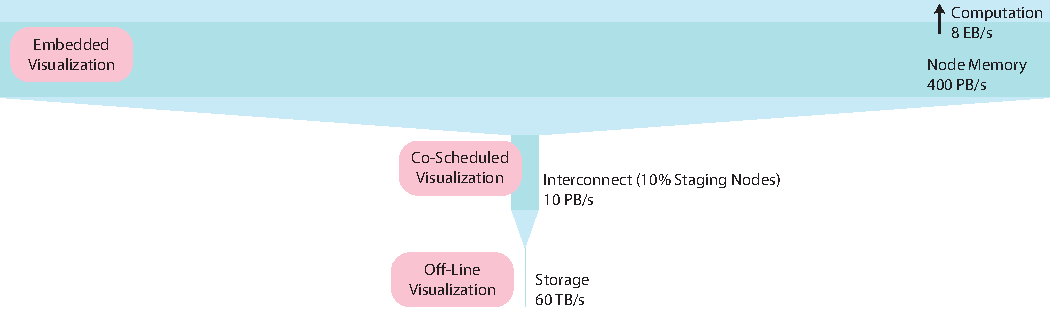
\includegraphics{images/MinardInSitu}
  \caption{Visual depiction of the relative bandwidth of exascale system
    components\lcite{ScientificDiscoveryExascale2011}.}
  \label{fig:IOBandwidths}
\end{figure*}

\subsection{Emerging Frameworks for Scientific Discovery at Exascale}

\noindent
DOE is currently addressing many of the programming challenges for exascale
through funding of various projects addressing different aspects of the
problem.  The first project, PISTON\lcite{PISTON}, facilitates the
development of visualization and analysis operators with highly portable
performance.  As noted previously, there is a wide variety in the hardware
and development environments for multithreaded environments, and PISTON
provides mechanisms both to compile across these development environments
and to run efficiently on many different devices.  It does this using a
data parallelism model and basic parallel operations much like that
proposed by Blelloch\scite{Blelloch1990}.

The second project, Dax\lcite{Moreland2011:LDAV}, simplifies the
development of parallel visualization algorithms.  It does so by allowing
developers to build algorithms out of worklets, which are functions that
implement an algorithm's behavior on an element of a mesh or a small local
neighborhood.  Worklets are designed in serial but can be concurrently
scheduled on an unlimited number of threads without the complications of
memory clashes or other race conditions.  Dax also provides many of the
basic topology structures and common operations on them to better
facilitate algorithm development.  It also allows algorithms to adapt to
memory structures of external applications without having to copy to a
different data structure\lcite{Moreland2012:PDAC}.

The third project, EAVL\lcite{EAVL}, updates the traditional data model for
modern simulation codes and investigates how the updated model can achieve
computational and memory efficiency.  EAVL defines more flexible mesh
structures, which more efficiently support many non-traditional types of
data such as for graphs, mixed data types, high-order fields, and adaptive
meshes.

See Sewell \etal\scite{Sewell2012} for a more in depth description of these
and other exascale-related projects.  The good news from these projects is
that they provide good introductory steps to implementing high-performance
visualization at exascale.  If successful, these changes should produce few
negative or even noticeable changes to the abilities of production
visualization software.

\section{Recording Results}
\label{sec:RecordingResults}

\noindent
Let us consider a different aspect of the exascale machine.  Consider the
change in the bandwidth to and from the storage system (bottom row of
Table~\ref{table:PetascaleVsExascale}).  Although the peak performance of
the computer should rise by three orders of magnitude, the bandwidth to the
storage only increases by one order of magnitude.  The consequence is that
a smaller fraction of results can be recorded when a simulation is run.

This is not a new trend in supercomputing.  For the last 20 years one could
expect each generation of supercomputer to have more floating point
operations per second and more concurrency, but comparatively less storage
and I/O bandwidth.  That is not to say that the storage systems have not
been improving; they have just been improving at a much slower rate than
the rest of the system.  As an example, two generations ago ASCI Purple, a
100 teraFLOP machine, had a peak bandwidth of 140~GB/s to its parallel
storage.  One generation ago, JaguarPF, a petaFLOP machine, had a peak
bandwidth of 200~GB/s to its parallel storage, which is not a dramatic
improvement.  To exacerbate the issue, few real applications are capable of
achieving anywhere near peak performance, and all applications must
sometimes deal with file system contention with jobs both on and off the
computer.

Thus, as simulations are scaled up on larger machines and perform
calculations at faster rates, there comes a time when it is impractical to
write results at a fast enough rate to do a proper analysis.  When this
time comes, we must become smarter about what gets written out and we must
move analysis closer to the data because there is no point in running a
simulation in the first place if we do not get the proper analysis out of
it.

\begin{table*}
  \centering
  \caption{List of visualization solutions with respect to coupling with a
    running simulation and their respective properties.}
  \label{table:InSituSolutions}
  \begin{tabular}{@{}lccccc@{}}
    \toprule
    & Capability & Coupling & Footprint & Transfer & Interactive \\
    \midrule
    Tightly Integrated & Low & Tight & \textcolor{goodcolor}{Low} & \textcolor{goodcolor}{None} & No \\
    Embedded & \textcolor{goodcolor}{High} & Tight & High & Possible memcopy & No \\
    Hybrid & \textcolor{goodcolor}{High} & Tight & Medium & Subset Hi Speed Transfer & \textcolor{goodcolor}{Yes} \\
    Co-Scheduled & \textcolor{goodcolor}{High} & \textcolor{goodcolor}{Loose} & Extra Nodes & Hi Speed Transfer & \textcolor{goodcolor}{Yes} \\
    Off-Line & \textcolor{goodcolor}{High} & \textcolor{goodcolor}{Loose} & \textcolor{goodcolor}{None} & \textcolor{badcolor}{Slow Persistent Storage Cost} & \textcolor{goodcolor}{Yes} \\
    \bottomrule
  \end{tabular}
\end{table*}

\subsection{Relative Data Bandwidth}

\noindent
Figure~\ref{fig:IOBandwidths} provides a Minard plot depicting the
bandwidths of different I/O components by the proportional width of their
respective blue bars.  (See Tufte\scite{Tufte2001} for a longer description
of Minard plots and their merits.)  Not shown on this plot is the rate at
which data can be computed.  At $10^{18}$ double precision floating point
operations per second, the exascale computer on aggregate will produce 8~EB
per second.  On this plot that would be almost 4 yards across.  The
aggregate bandwidth of the local memory --- that is, the speed at which
data can be pulled from memory to a local process summed over the entire
machine --- is 400~PB/s.  This is as fast as we can reasonably expect to
access data on the system, but it is only available in the same job space
as the running simulation.  If we were to offload that data to another job,
say a staging job running on a generous allocation of 10\% of the overall
nodes, then we could stream the data to this job at 10~PB/s, which is
pretty fast but only 2.5\% the local access rate.  Furthermore, one must
worry about the limited memory available on the staging nodes.  To move the
data entirely to disk storage, the bandwidth drops way down to 60~TB/s.
This is only 0.015\% the rate at which data can be written to local memory
and only 0.00075\% the rate at which data can be computed.  So, only an
extremely small fraction of data can ever hope to be captured on disk.

The problem, of course, is that the majority of visualization and analysis
done today is performed ``off-line'' after the data has been written to
disk.  Off-line visualization offers many advantages that make it the
easiest way to perform visualization.  First, it makes the interface
between simulation and visualization simple.  The visualization needs only
to understand the format used when the simulation writes the data to disk.
Second, it makes scheduling and performing the visualization, particularly
when done by a human, much easier.  The visualization job can be scheduled
completely independently of the simulation and at a time most convenient
to the user.  Third, the results data are placed in persistent storage, so
any analysis not performed immediately can be done at a later time if they
are later deemed necessary.

None of these advantages mean anything, however, if it is not possible to
get the necessary data to the storage system.  In the case where there is
not sufficient bandwidth to store raw results from the simulation, then the
visualization must be moved ``closer'' to the visualization (upwards in the
Minard plot of Figure~\ref{fig:IOBandwidths}).  You could co-schedule a
visualization job at the same time as the simulation job and set up a
transfer mechanism over a high speed network.  If that still is not enough
bandwidth, you could embed the visualization directly in the simulation so
that the visualization has direct access to the data while it is still in
local memory.

\subsection{Gamut of Coinciding Visualization Solutions}

\noindent
Given the fact that the bandwidth to results data increases as we move
closer to the visualization, it is reasonable to ask why we would not
always choose to embed directly with the simulation.  Although this would
certainly optimize the bandwidth to the data, moving visualization closer
to simulation comes at a cost.

The first cost is that of complexity in development.  Creating a
visualization that can be co-scheduled requires a complex connection
between the simulation and visualization and generally requires a fully
featured I/O system to manage it.  The co-scheduled visualization also
requires added complexity in the job scheduler of the parallel computer.
Embedding a visualization in a simulation requires a complete integration
of simulation and visualization codes.  In practical terms, it means that
both development teams must work together, which tends to involve crossing
several cultural barriers.

The second cost is that of loss in functionality.  Once we move our
visualization away from off-line, the data we work with becomes transient.
A co-scheduled visualization has access only to data that is locally
available, which may be no more than one snapshot in time.  Once the
visualization moves on to another snapshot in time, or if the simulation
passes a snapshot in time before the visualization is ready, that data is
lost forever.  An embedded visualization has the further constraint that
whatever operations are to be performed, they have to already be declared
when the simulation is ready to invoke them.

Consequently, there is no simple single solution that can address all of
our current or projected visualization coupling needs.  Our group has
experimented with an entire spectrum of solutions and found each one to
have its own advantages and disadvantages as summarized in
Table~\ref{table:InSituSolutions}.

On one end of the spectrum we can have a very tightly integrated
visualization component built from the ground up for a specific need in a
simulation.  Such a targeted solution can have a very small footprint as it
can make specialized optimizations for the particular data types and
representations used.  Such a solution can be perfect for an analysis team
that wants a specific, targeted, and fairly simple functionality.  However,
in our experience a successful integration usually begets further requests
for new features, which would be readily available in a more
general-purpose library.  Hence, the tightly integrated approach often
spirals into a large duplication of efforts between projects, and we try to
avoid it.

A preferred method, from the visualization software developer's standpoint,
is to embed a general-purpose visualization library into a
simulation\lcite{Fabian2011,VisItLibsim}.  Once integrated, the simulation
now has access to all the visualization capabilities of the visualization
library as well as possible integration with already familiar visualization
tools.  The disadvantage of such an approach is that the footprint of such
a library tends to be high, especially when dynamic selection of
visualization capabilities is supported.  Also, it means that any
visualization algorithm used must scale to the same job size as the
simulation it is embedded in, which can be challenging\lcite{Fabian2012}
although also useful outside the simulation.

Co-scheduled visualization (also often called \intransit visualization)
alleviates some of the problems of embedded
\insitu\lcite{Moreland2011:PDAC,Biddiscombe2012,Klasky2011}.  The coupling
between visualization and simulation can be simplified by connecting them
indirectly through an I/O layer although general-purpose I/O layers are
still in development.  Also, the co-scheduled visualization job can provide
an entire suite of visualization tools without directly adding to the
footprint of the simulation although it does require a sufficiently large
separate allocation of nodes on the same computer or nearby.  A
disadvantage of the co-scheduled method is that an overhead is incurred for
transferring the data from simulation job to visualization job, but once
that is done the two processes can execute asynchronously, further
eliminating some of the overhead in the simulation.

In some circumstances we have found a hybrid method between embedded and
co-scheduled visualization is useful.  In this method, a visualization
component is directly embedded in the simulation, but the visualization can
also connect and transfer data to a separate and smaller visualization
job\lcite{Moreland2011:PDAC}.  The intention here is to provide a tightly
coupled and highly scalable algorithm directly in the simulation code that
can quickly extract salient information and pass this reduced data to
another process.  This second process can then be used to serve an
interactive visualization to a user without blocking the large simulation.

\section{Other Exascale Challenges}
\label{sec:Other}

\noindent
So far we have considered some of the most urgent problems facing us for
exascale computing and the ones we are directly working on at Sandia
National Laboratories.  There are, however, many more challenges that face
us as we approach exascale, and this section gives a brief overview of some
other important issues.

\subsection{Resilience}

\noindent
Although our production scientific-visualization tools are designed to
provide reliable operation, resilience has not been the primary concern for
their development.  Should a problem occur during visualization, such as a
hardware failure, that causes a catastrophic interruption, it is of
relatively little consequence to simply restart the visualization and
reload the data when running in off-line mode.  However, things can change
dramatically for exascale.  When running \insitu at the exascale, it is
vital that the visualization components be robust.  It is not looked upon
favorably when visualization brings down a large simulation job.

At exascale we expect failures to occur more frequently as well.  The
exascale computer comprises significantly more hardware components.  More
components means a greater chance that one will fail, which means that the
mean time to failure goes down.  When the mean time to failure drops low
enough, even independent visualization jobs need to consider resiliency.

In addition to more likely catastrophic failures, high-performance
computing may need to be adept at handling soft errors, which are errors
such as small data corruption that are never detected.  Soft errors are
more likely at the exascale not only due to the greater number of
components but also because some error detecting hardware may be removed in
an effort to reduce the power consumed.

Ultimately, the operation of an exascale computer may be less deterministic
than what we currently expect of a petascale computer.  Not only must our
code be able to operate under uncertainty, but it must also be able to
characterize the uncertainty in the data that it produces.

\subsection{Compression and Extraction}

\noindent
As described in Section~\ref{sec:RecordingResults}, less results data can
be captured from a simulation.  Ultimately, this means that we must make
better use of the bandwidth that we do have available by providing more
information with less data.  One straightforward way to do this is to
compress the data.  Data compression has a long and fruitful history, but
scientific analysis and visualization provides several new challenges.
Scientific data tends to be of floating point numbers with well defined but
possibly complicated and irregular structure, which is different from most
other uses of compression.  Furthermore, we could benefit from both
lossless and lossy compression, but for lossy compression it is very
important to be able to both constrain and characterize the inaccuracy
introduced by lossy compression.

Another approach to reducing the amount of data returned is by extracting
exactly the information desired.  One direct method of extraction is to
perform a feature characterization and write out properties of features.
The challenge of this approach is that feature characterization is very
specific to a particular scientific domain and analysis.  Furthermore,
features are often difficult to specify let alone extract, and often feature
identification is an expensive operation.

\subsection{Provenance}

\noindent
Provenance provides a record of what operations and parameters produced a
given set of data.  Recent works of provenance in scientific visualization
systems record the set of parameters used to build a visualization and the
history of exploration to get there\lcite{JankunKelly2002,VisTrails}.

With the added focus of \insitu visualization at the exascale, provenance
takes on a new and important role.  Because data is transient, it becomes
impossible to revisit old data and verify old visualization results.  To
maintain confidence in the data analysis without the original data, it is
important to capture what methods were used to draw any set of
conclusions.

\subsection{Uncertainty Quantification}

\noindent
As the computational power of supercomputers increases, we expect greater
efforts to be made in tracking uncertainty and quantifying the uncertainty
in simulations.  However, this uncertainty quantification is of little use
if the analysis can provide no insight into the envelope of possible
values.  Visualization systems need to incorporate uncertainty in their
visual representation of data\lcite{Potter2012}.

\section{Final Remarks}
\label{sec:Conclusion}

\noindent
The transition from petascale to exascale computing is an exciting time for
all aspects of high-performance computing.  A fundamental shift in the
basic computer architecture of our machines presents a great many
challenges for scientific visualization as well as all other large-scale
applications, but it also presents us with numerous opportunities as well.
Exascale promises major advances in computing ability, which, if properly
harnessed, can provide major advances in science.

One interesting upshot of the exascale challenge is that it brings
researchers from different disciplines together.  Because the engineering
decisions for the design of every part of the system from the hardware to
the application are so interconnected, the study of exascale has lead to
several codesign centers that share system problems and solutions to
mutually design the entire system.  More pervasively, we find that moving
to exascale requires us to transition from a technology-driven science,
where one focuses on the computational tools, to a discovery-driven
science.  Discovery-driven science dictates that the primary focus of a
scientific endeavor be the end goal and the scientific discoveries we need
to make.  With it, we holistically consider the entire computational
experiment design rather than a series of mutually exclusive steps.

\section*{Acknowledgments}

\noindent
This report is a summary of ongoing work by a great number collaborators
over many institutions.  In particular, I would like to thank the
following: Nathan Fabian and Ron Oldfield from Sandia National
Laboratories; Kwan-Liu Ma, Robert Miller, and Yecong Ye from the University
of California at Davis; Berk Geveci, Utkarsh Ayachit, Robert Maynard, Brad
King, Andrew C. Bauer, Pat Marion, Sebastien Jourdain, David DeMarle, and
David Thompson at Kitware, Inc.; James Ahrens and Jonathan Woodring at Los
Alamos National Laboratory; Scott Klasky and Norbert Podhorszki at Oak
Ridge National Laboratory; Venkatram Vishwanath, Mark Hereld, and Michael
E. Papka at Argonne National Laboratory; Michel Rasquin and Kenneth
E. Jansen at the University of Colorado at Boulder; Ciprian Docan and
Manish Parashar at Rutgers University.


This work was supported in part by the Director, Office of Advanced
Scientific Computing Research, Office of Science, of the U.S. Department of
Energy under Contract No. 12-015215, through the Scientific Discovery
through Advanced Computing (SciDAC) Institute of Scalable Data Management,
Analysis and Visualization.

This work was supported in part by the DOE Office of Science, Advanced
Scientific Computing Research, under award number 10-014707, program
manager Lucy Nowell.

Sandia National Laboratories is a multi-program laboratory operated by
Sandia Corporation, a wholly owned subsidiary of Lockheed Martin
Corporation, for the U.S. Department of Energy's National Nuclear Security
Administration.

\noindent
{\small SAND 2013-0180C}

\bibliographystyle{IEEEtranS}
\bibliography{OhShExascale}

\end{document}
